\chapter{绪论}
\section{研究背景和意义}
近年来深度学习技术快速发展,在图像识别\cite{krizhevsky2012imagenet}、自然语言处理\cite{brown2020language}、自动驾驶\cite{teichmann2018multinet}、医疗诊断\cite{gulshan2016development}等领域取得了显著的进展和广泛的应用。现阶段的深度学习算法在准确性上已经可以达到很好的效果,但仍普遍存在过度自信问题(Overconfident issue),即深度神经网络对其预测结果上往往过于自信,即使在它不熟悉的输入上,也可能错误地给出过高的预测概率。在一些高风险的领域,比如医疗诊断,自动驾驶等,一次错误的预测可能会带来严重的后果,过度自信问题使得神经网络在这些领域的应用仍然受到限制。因此,在实际应用中不仅需要模型能准确给出预测结果,还希望模型能给出一个值指示本次预测结果可靠程度,这就是神经网络的\textbf{不确定性(Uncertainty)}。神经网络的本次预测不确定性高,就可以在必要时引入人类监督或放弃高风险决策,规避风险和灾难性后果。

对神经网络不确定性的研究在实际应用中具有重大意义,不确定性量化(Uncertainty Quantification,UQ)有助于提升模型的鲁棒性,帮助模型更稳健、更可靠地应用于实际任务。通过对输入数据的不确定性建模,神经网络可以更加适应不同的输入分布,从而提高在开放环境中的表现,在面对异常数据或分布外数据(OOD,Out-of-Distribution)时能够可靠地做出应对。在实际应用中,不确定性量化帮助模型识别它对某些输入的预测信心不足的情况,避免错误决策引发的系统事故。另一方面,神经网络不确定性的研究对神经网络的可解释性也有重要意义,通过研究不确定性,学术界和工业界能够更深入地理解神经网络的行为和特性。当前多数研究和应用都把神经网络作为“黑箱”模型,其缺乏可解释性的问题长期以来阻碍了其在关键领域的应用。通过不确定性研究,模型可以对自己的预测进行自我评价,为用户提供更直观的信心指标。这不仅有助于用户更好地理解和使用神经网络系统,还能增加对人工智能技术的信任。当前,不确定性研究已经催生了许多新的方法,例如深度高斯过程、贝叶斯神经网络、蒙特卡罗随机失活(MC dropout)、对抗训练等。这些方法不仅拓展了神经网络的理论基础,也为其他机器学习问题(如模型选择、主动学习)提供了新思路。例如在人机协作系统中,提供置信度信息可以增强用户对模型的信任,有效指导主动学习和数据采集。

\section{不确定性的来源与分类}
\textbf{神经网络不确定性(Uncertainty in Neural Networks)}是指在神经网络的预测中,描述其对预测结果的置信程度或潜在预测错误的能力\cite{abdar2021review}。神经网络的不确定性量化在许多实际应用中非常重要,尤其是在需要高可靠性和安全性的领域,如自动驾驶、医疗诊断和金融预测\cite{gawlikowski2023survey}\cite{he2023survey}\cite{gal2016uncertainty}。在实际应用中,神经网络中的不确定性通常可以分为两类\cite{abdar2021review}:\textbf{模型不确定性}(Model Uncertainty)和\textbf{ 数据不确定性}(Data Uncertainty)。

\textbf{模型不确定性},又称为\textbf{认知不确定性}(Epistemic Uncertainty),表示所训练的神经网络模型本身能力的局限性,可能来源于模型结构,训练过程,训练数据不足。当训练数据不足时,模型的参数未能很好地捕捉数据分布分布,导致预测的结果含有很大的模型不确定性。模型不确定性可以通过改变训练模型,优化训练过程,增加训练数据来减少。如图\ref{fig:uncertainty},在训练数据以外所呈现的高不确定性是模型不确定性。\textbf{数据不确定性}(Data Uncertainty), 又称为\textbf{偶然不确定性}(Aleatoric Uncertainty),通常是由数据本身的随机性或噪声引起,可能来源于数据收集时噪声,数据标注时的错误。数据不确定性无法被消除。如图\ref{fig:uncertainty},训练数据本身所存在的误差和噪声引起的不确定性是数据不确定性。

数据不确定性和模型不确定性并非绝对的,有时候二者可以相互转化\cite{hullermeier2021aleatoric}。Valdenegro-Toro等人\cite{valdenegro2022deeper}也在研究中发现,在解耦不确定性的过程中,模型不确定性和数据不确定性会相互影响,这一点是出乎意料的,因为通常认为只有模型不确定性应该与模型交互,而数据不确定性则不应和模型有关。

\begin{figure}[H]
    \centering
    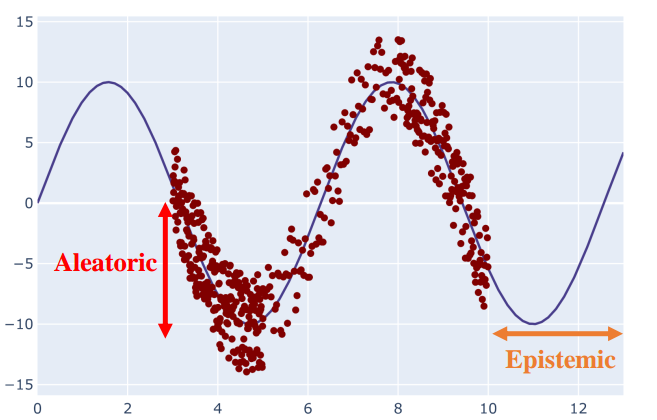
\includegraphics[width=0.9\linewidth]{assets/1-1.png}
    \caption{不确定性的来源与分类\cite{abdar2021review}
}
    \label{fig:uncertainty}
\end{figure}

\section{不确定性研究的应用}
神经网络的不确定性研究(Uncertainty in Neural Networks)在许多应用场景中都具有重要价值,特别是在需要对预测结果的可靠性、稳定性和信心进行量化的任务中。传统的神经网络通常给出一个确定的预测结果(例如,分类标签或回归值),但并没有提供关于该结果的不确定性信息。而不确定性建模则能够量化模型对其预测的信心程度,这在多个领域中具有广泛的应用。

1. 自动驾驶

在自动驾驶系统中,车辆必须能够做出实时决策,基于摄像头图像、雷达、激光雷达等数据预测和识别路况。然而,这些数据本身可能存在噪声,或者在复杂环境中不完全可靠。通过不确定性建模,自动驾驶系统可以识别哪些预测是可靠的,哪些可能需要进一步验证或修正。决策制定时结合不确定性,可以优先选择对结果不确定性较低的路径规划或行动,对不确定性较高的引入人的干预。近年来关于神经网络不确定性和自动驾驶领域的结合出现很多研究,Di Feng, Lars Rosenbaum等人\cite{feng2018towards}针对激光雷达(LiDAR)的3D车辆检测任务,提出了一种结合贝叶斯深度学习的方法,能够同时估计数据不确定性和模型不确定性,通过不确定性信息优化预测结果,增强了自动驾驶系统在复杂环境中的安全性和稳健性。Hujie Pan等人\cite{pan2020towards}针对激光雷达(LiDAR)的3D车辆检测任务,结合不确定性估计方法,对回归的坐标引入拉普拉斯分布,设计了一种改进的损失函数,以获得更具有解释性和可靠性的预测结果。SalsaNext\cite{cortinhal2020salsanext} 是一种针对自动驾驶领域设计的高效、不确定性感知的语义分割模型,用于处理 LiDAR 点云数据。它在原有 SalsaNet\cite{Aksoy2019SalsaNetFR}的基础上进行了改进,结合了注意力机制和贝叶斯学习框架,实现了更高的精度和不确定性估计能力,为自动驾驶中的环境感知提供了可靠的解决方案。赵洋\cite{QCYK202405002}深入研究了自动驾驶目标检测中不确定性估计的方法,利用不确定性信息来提高目标检测的准确性,并总结了不确定性估计的评价指标。

2. 医疗诊断

在智能辅助诊断领域,尤其是在面对复杂或模糊的医学影像时,对不确定的研究能够为医生提供关于某项影像诊断的置信度,帮助医生判断是否需要进一步的检查或其他医学手段。在疾病预测方向上,基于患者历史数据和医学影像,模型预测某种疾病的风险,并通过不确定性量化本次预测的可信度,对不确定度高的预测引入专业医生的判断,可以减少误诊率,降低医疗事故的可能性。在医学图像检测或者分割任务中,某些图像可能很模糊,此时模型不仅需要做出准确的预测,还需要能够提供关于其预测结果不确定性的估计,通过不确定性估计,模型可以指出分割结果的可靠区域,辅助医生进行更准确的解读。不确定性在医疗诊断领域应用上的研究,Guotai Wang等人\cite{wang2019aleatoric}研究如何结合测试时增强的方法,对卷积神经网络进行不确定性估计,从而提高医学图像分割的鲁棒性。Tanya Nair等人\cite{nair2020exploring}针对病变检测和分割,提出了一种改进的U-Net架构,结合了四种不确定性度量:预测方差、蒙特卡罗样本方差、预测熵和互信息,辅助识别模型在预测中的不确定区域,提高病变分割的准确性。邹可\cite{1024642336.nh}通过证据不确定性估计方法的研究,将不确定性估计应用到医学分割领域,提高了医学图像分割的准确性和可靠性。


3. 金融风控与预测

在金融行业中,不确定性量化有助于提高风险管理和预测系统的可靠性,尤其是在面对市场波动和不确定环境时。在信贷风险评估上,通过不确定性量化,金融机构能够识别贷款申请中哪些因素对违约预测有较高不确定性,从而采取更谨慎的风险管理措施。在市场预测上,量化市场趋势预测中的不确定性,可以帮助投资者做出更明智的决策,尤其在市场波动较大的情况下。在金融行业中,关于不确定性的研究,WONG S Y等人\cite{wong2025quantifying}研究了不确定性量化对复杂金融时间序列预测的必要性,聚焦于时间序列中的波动性聚集特性(如资产回报率预测),提出了一种结合模型集成和证据网络的方法,显著提高了金融市场中加密货币和股票的预测的不确定性量化效果。

4. 自然语言处理

在自然语言处理任务中,神经网络通常需要处理复杂的文本和语言,不仅要生成准确的输出,还要提供预测的不确定性。例如,在机器翻译、情感分析或问答系统中,了解模型对预测结果的置信度对于理解其输出的可信度非常重要。在机器翻译领域,模型可以提供翻译的置信水平,帮助用户理解哪些翻译结果可靠,哪些可能需要进一步验证。在情感分析领域,评估情感分析模型的预测可信度,帮助商家了解用户评论中的潜在情感。在自动问答系统中,不确定性建模可以提供关于某个答案的置信度,帮助系统在遇到不确定的答案时请求进一步的信息或向用户确认。在自然语言处理领域关于不确定性的研究,郭晓亭\cite{1022812574.nh} 设计了一种不确定性感知的损失函数,提高了文本情感分析准确性。X. Han等人\cite{han2019attention} 提出一个基于注意力机制的神经网络框架,识别社交媒体文本中的不确定性。近年来大语言模型的兴起和广泛应用,也催生了关于不确定性在大模型方向上的研究。Lorenz Kuhn等人\cite{kuhn2023semantic}介绍了一种用于衡量大语言模型不确定性的方法,对于像问答任务这样的应用,作者提出了“语义熵”概念,通过广泛的消融实验,作者证明了语义熵在问答数据集上的表现优于其他对比基准,能够更有效地预测模型的准确性。Zhen Lin\cite{lin2024generating}针对大型语言模型(LLMs)在自然语言生成任务,特别是在黑箱模型的场景下,提出了多种不确定性量化指标,筛选不可靠的结果或将其交由人工进一步评估。

% 5. 机器人与自主系统

% 深度学习在机器人领域面临独特挑战,例如测试条件与训练分布不一致可能导致性能下降。因此,研究如何量化神经网络预测的不确定性,以避免灾难性错误,对于推动机器人技术的发展尤为重要。在路径规划与控制方面,通过不确定性量化,机器人可以识别哪些路径或动作是更安全的,哪些决策可能会导致更高的风险。在环境感知方向上,在复杂环境中(例如多变的室内环境或户外环境),机器人可以基于不确定性评估来选择更可靠的传感器数据进行决策。有关不确定性量化在机器人方向上的研究,Peretroukhin, Valentin and Giamou\cite{peretroukhin2020smooth}引入了一种概率分布表示,将旋转表示和不确定性建模相结合,可以更准确地学习旋转,同时提供对模型置信度的估计,从而在姿态估计和物体跟踪任务中表现更出色。。Yang等人\cite{yang2020d3vo}的研究通过联合学习场景深度、相机位姿以及不确定性估计,构建了一个端到端的框架,通过引入不确定性评估以增强对环境变化的适应性。


\section{研究内容}
% 本文主要研究对象是神经网络的模型不确定性量化问题,当前综合来看最优的不确定性建模方法是模型集成的方法,但是这种方法因为需要训练和存储多个网络,所以存储和计算复杂度较高。为了更高效地建模不确定性,本文的研究思路基于高维特征的概率密度建模不确定性,该方法只需要单个确定的神经网络即可建模神经网络的模型不确定性。具体而言,基于高维特征概率密度建模不确定性,是通过对训练集上神经网络提取的高维特征进行概率密度建模,当一个新的测试输入进入神经网络,所得到的新的高维特征在所建模的分布上计算出一个概率密度,作为模型对测试输入不确定性的度量。这种模型不确定性建模的思路,在DDU算法\cite{Mukhoti_2023_CVPR}中被提出并研究,但是实验发现DDU算法相比当前最优方法模型集成在不确定性建模效果上仍有一定差距,因此,本文的研究核心是在DDU算法的基础上,进一步研究基于高维特征概率密度的方法建模不确定性,并改进该思路对神经网络模型不确定性的建模效果,在OOD检测,对抗样本识别,主动学习等代理任务上评估所提出的改进的效果。

% 本文的研究工作从两个方面展开。首先,通过计算输出对输入图片的梯度并绘制梯度响应图,观察到分布外样本和训练集样本存在着明显的分布差异,并通过理论分析证明这一实验现象。之后提出把梯度信息作为扰动加入到输入图片中,然后重新计算出概率密度,理论分析证明了加入梯度相关的扰动能拉大分布内样本和分布外样本分布的差异,可以提升对不确定性的建模效果,最后在OOD检测,对抗样本识别,主动学习等任务上的评估该改进方法,可以加入输入扰动能提升基于高维特征概率密度建模不确定性的效果。

% 另一方面,本文通过对特征空间的分析指出,提升特征空间的类内紧密性和类间可分性可以提升高维特征概率密度建模不确定性的效果,进而基于度量学习的思路,提出一种新的辅助损失函数,和交叉熵损失函数联合训练,并在联合训练后的特征空间上建模概率分布,使用概率密度表征模型不确定性。通过对联合训练后特征空间的定量分析,联合训练提升了特征空间的类内紧密性和类间可分性,最后在OOD检测任务上、误分类样本识别等任务上进行评估,可以看到联合训练的方法能提升基于高维特征概率密度建模不确定性的效果。在这一部分,为了解决特征维度太高而导致的存储难题,提出使用主成分分析对高维特征降维,在降维后的特征空间上建模分布并计算不确定性,理论和实验都表明这一策略极大的减少了高维特征的存储空间。

% 本文研究内容和创新点概括如下:
% \begin{itemize}
%     \item 实验观察到概率密度关于输入的梯度在训练集样本和分布外样本存在明显的差异,并从理论上分析证明
%     \item 对输入图片添加梯度有关的扰动,拉大分布内样本和分布外样本的分布差距,提升模型不确定的建模效果
%     \item 融合度量学习的思想,提出新的辅助损失函数和交叉熵损失函数一起联合训练
%     \item 使用主成分分析对高维特征降维,降低存储复杂度
% \end{itemize}


本文主要研究神经网络模型不确定性的量化问题。目前,综合来看,最优的不确定性建模方法是模型集成方法。然而,这类方法需要训练和存储多个网络,导致存储和计算复杂度较高。为实现更高效的不确定性建模,本文采用基于高维特征概率密度建模的不确定性量化方法,仅通过单个确定性神经网络即可对模型的不确定性进行建模。具体而言,该方法通过对训练集中神经网络提取的高维特征进行概率密度建模,当新的测试输入进入网络时,计算其对应高维特征在所建模分布上的概率密度,以此作为模型对该测试输入不确定性的度量。

基于高维特征概率密度建模的不确定性这一思路最早在DDU算法\cite{Mukhoti_2023_CVPR}中被提出并研究。尽管该算法在不确定性建模方面取得了一定效果,但实验表明,与当前最优的模型集成方法相比,DDU算法仍存在差距。因此,本文以DDU算法为基础,进一步研究基于高维特征概率密度的方法以提升不确定性建模效果,并在域外样本检测、对抗样本识别和主动学习等代理任务上验证所提出改进方法的有效性。


本文的研究内容主要包括两个方面,其一,通过计算输出对输入图片的梯度并绘制梯度响应图,实验观察到分布外样本和分布内训练样本的梯度分布存在显著差异,分布外样本的梯度响应显著更大。基于这一发现,本文提出将梯度相关的信息作为扰动引入到输入图片中,并重新计算其概率密度。理论分析表明,加入梯度相关扰动能够有效拉大分布内样本和分布外样本的分布差距,从而提升不确定性建模的效果。通过在OOD检测、对抗样本识别和主动学习等任务上的实验评估,结果表明加入输入扰动可以显著提升基于高维特征概率密度建模的不确定性效果。

其二,本文通过对特征空间的分析指出,提升特征空间的类内紧密性和类间可分性能够显著改善高维特征概率密度建模的不确定性效果。基于度量学习的思想,本文提出了一种新的辅助损失函数,并将其与交叉熵损失函数结合进行联合训练。在联合训练后的特征空间中建模概率分布,并使用概率密度量化模型不确定性。通过对联合训练后的特征空间进行定量分析,结果表明联合训练显著提升了类内紧密性和类间可分性。在OOD检测、误分类样本识别等任务中的评估结果进一步验证了联合训练方法能够有效提升基于高维特征概率密度的不确定性建模性能。此外,为解决高维特征导致的存储复杂度问题,本文提出使用主成分分析对高维特征进行降维。在降维后的特征空间上进行概率分布建模不仅能够显著降低存储需求,同时还提高了建模效率和效果。理论与实验均证明了这一策略的有效性。


本文的研究内容与创新点总结如下:
\begin{itemize}
    \item 实验观察到概率密度关于输入的梯度在分布内样本和分布外样本之间存在显著差异,并通过理论分析进行了验证。
    \item 提出基于输入图片添加梯度相关扰动的方法,能够拉大分布内样本和分布外样本的分布差距,从而提升不确定性建模效果。
    \item 基于度量学习思想,提出一种新的辅助损失函数,与交叉熵损失联合训练,以优化特征空间的类内紧密性和类间可分性。
    \item 使用主成分分析对高维特征降维,显著降低存储复杂度的同时提升建模效率与效果。
\end{itemize}



\section{章节安排}
本文共分五章内容组织。

第一章主要是对不确定性的介绍,介绍了不确定性的定义、来源与分类,不确定性研究的意义和相关应用。

第二章介绍了当前主流的建模不确定性的思路,主要包括贝叶斯神经网络,模型集成的方法,测试数据增强,单一确定性网络建模的方法,并介绍了这些方法是如何计算不确定性的。由于在实际场景中缺乏不确定的标注,所以直接评估不确定性建模效果是很困难的,在第二章最后介绍一般是如何通过OOD检测、误分类样本识别、主动学习等任务间接评估不确定性的建模效果。

第三章主要介绍了基于输入扰动的改进,首先是对梯度空间的分析,指出分布外样本和分布内训练样本的梯度分布存在显著差异,分布外样本的梯度响应显著更大,通过理论分析证明这一结论。基于此,在这一章提出将梯度相关的信息作为扰动引入到输入图片中,加入梯度相关扰动能够有效拉大分布内样本和分布外样本的分布差距,最后在OOD检测、误分类样本识别等代理任务上验证了改进后的方法对不确定性的建模效果的提升。

第四章主要介绍了使用辅助损失函数联合训练的改进,首先是对特征空间的分析,指出提升特征空间的类内紧密性和类间可分性能够显著改善高维特征概率密度建模的不确定性效果,进而提出一个新的辅助损失函数和交叉熵损失函数一起联合训练,为了减少模型存储还提出了对高维特征使用主成分分析降维,最后在OOD检测等任务上评估了改进后的方法的建模效果。

第五章是对本文研究的总结和对神经网络不确定性研究的未来的展望。
